\begin{figure}[H]
\centering
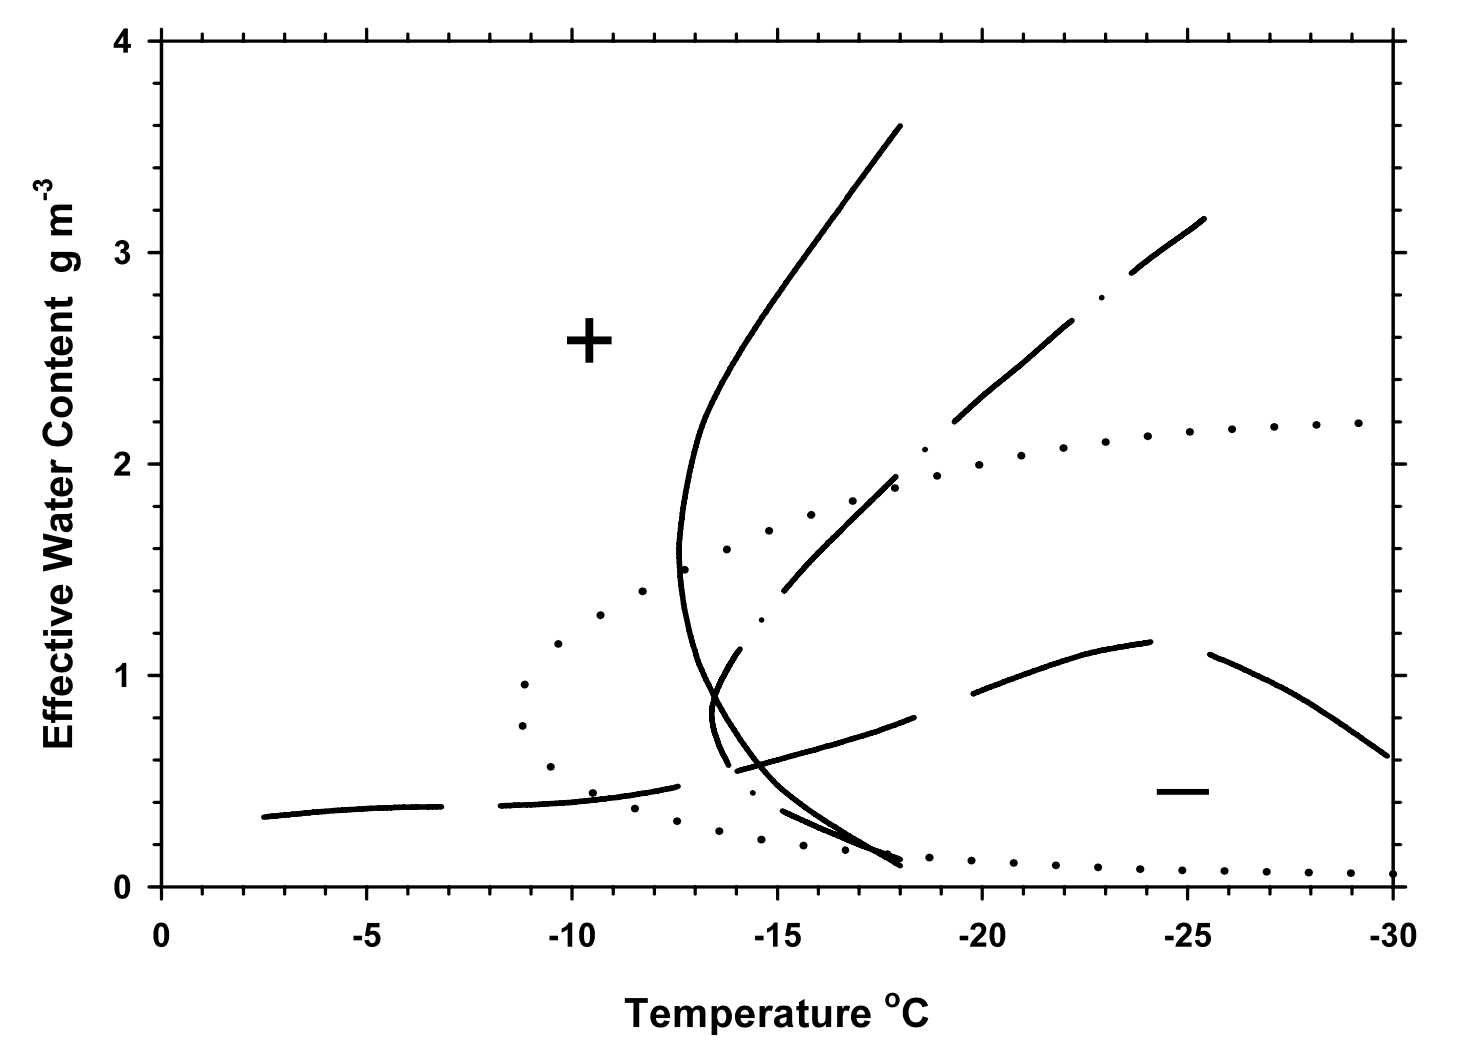
\includegraphics[width=0.7\textwidth]{charge_reverse_curves}
\singlespacing
\caption{\textit{Rimer charge sign boundaries from various laboratory studies. $\cdots$ \cite{takahashi1978riming}, $--$ \cite{saunders1998laboratory}, $-\cdot-$ \cite{pereyra2000laboratory}, $-$ \cite{saunders2006laboratory}. (\cite{saunders2008charge}, Fig. 12)}}
% \vspace{-50pt}
\label{fig:ChargeSign}
\end{figure}

\begin{figure}[H]
\vspace{40pt}
\centering
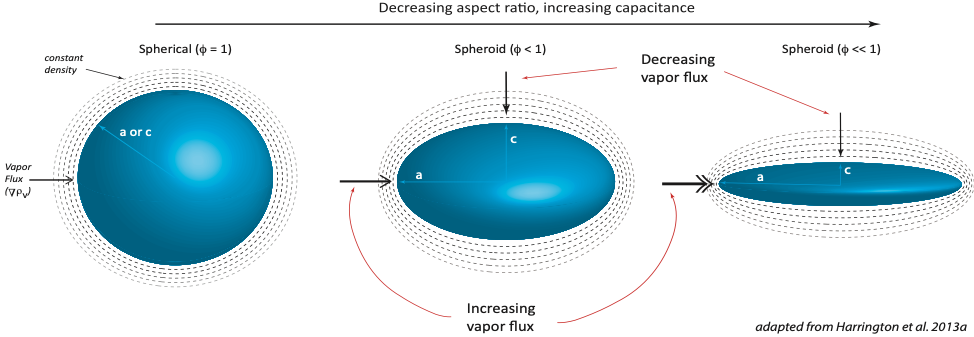
\includegraphics[width=\textwidth]{IceHabbit}
\singlespacing
\caption{\textit{Evolution of ice aspect ratio ($\phi=\frac{c}{a}$) as represented by spheroids. As aspect ratio evolves away from spherical, vapor density gradients concentrate over the area of greatest curvature. (\cite{harrington2013methoda}, Fig. 2)}}
\label{fig:icehabit}
\end{figure}

\begin{figure}[H]
\vspace{-20pt}
\centering
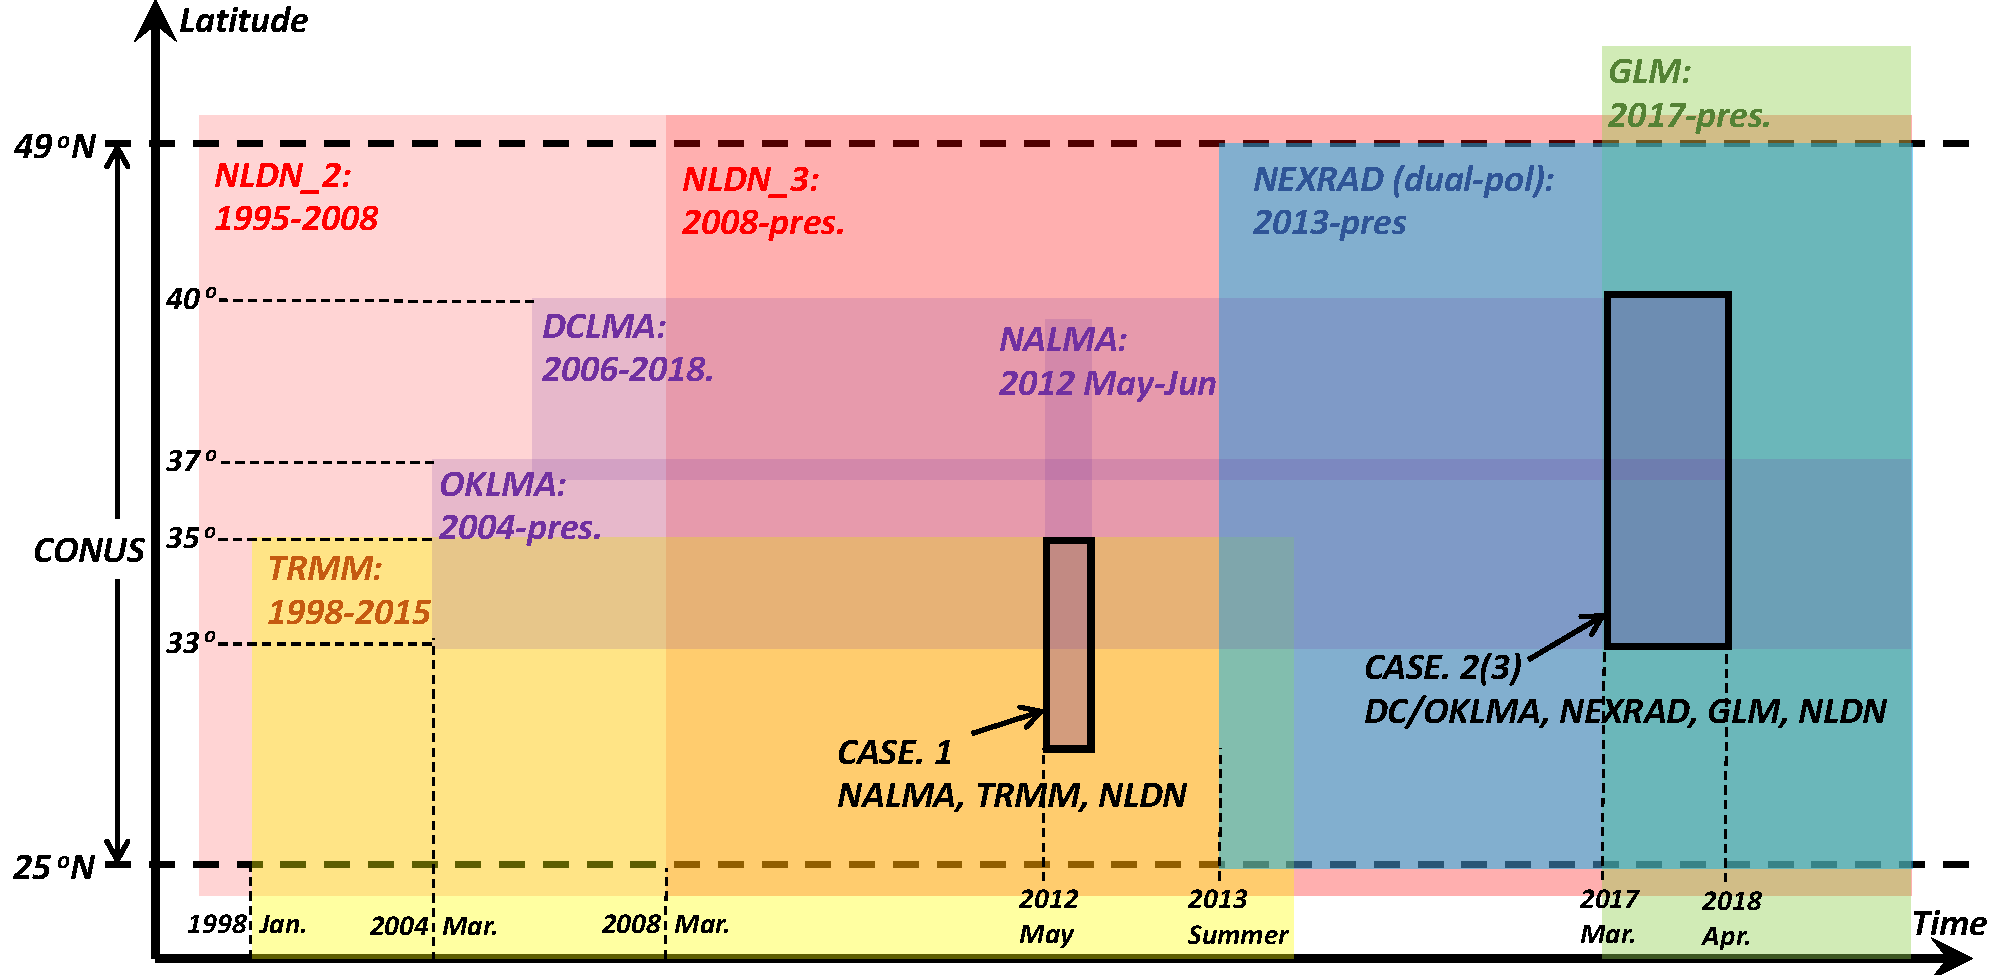
\includegraphics[width=\textwidth]{data_timeline}
\singlespacing
\caption{\textit{Schematic Temporal and Spatial (Latitude) Overlaps of Datasets and potential case selection ranges}}
\label{fig:data_timeline}
\end{figure}

\begin{figure}[H]
\vspace{-10pt}
\centering
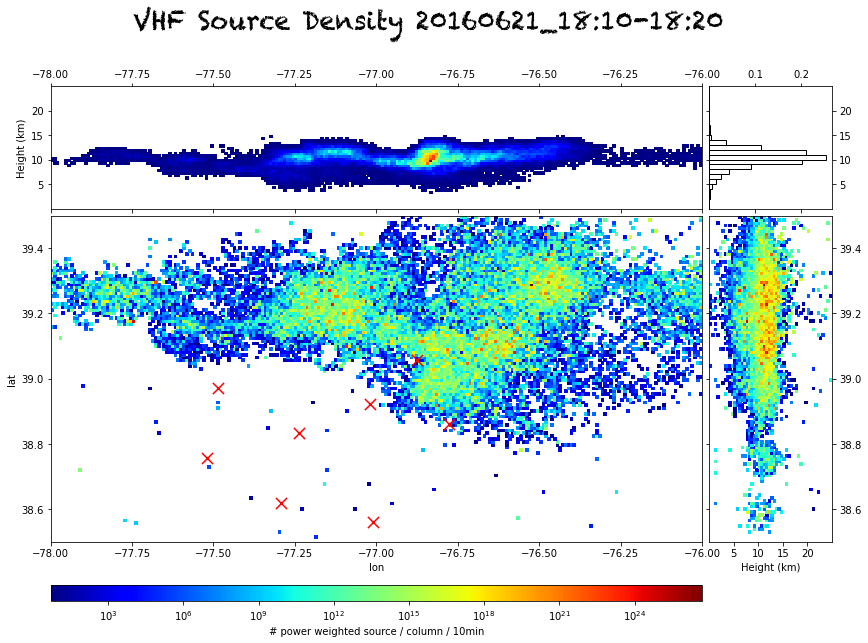
\includegraphics[width=0.75\textwidth]{dclma}
\singlespacing
\caption{\textit{DC-LMA derived 3-view distribution of Very-High-Frequency sources emitted by lightning occurred during June 21st 18:10-18:20 period, summed into ~0.75km(x)*0.75km(y)*0.5km(z) gridbox, weighted by power of radiation. Red crosses in lower left represent active detection cites, upper right patch is the probability of source occurrence in each 1-km level}}
\label{fig:dclma}
\end{figure}

\begin{figure}[H]
\vspace{40pt}
\centering
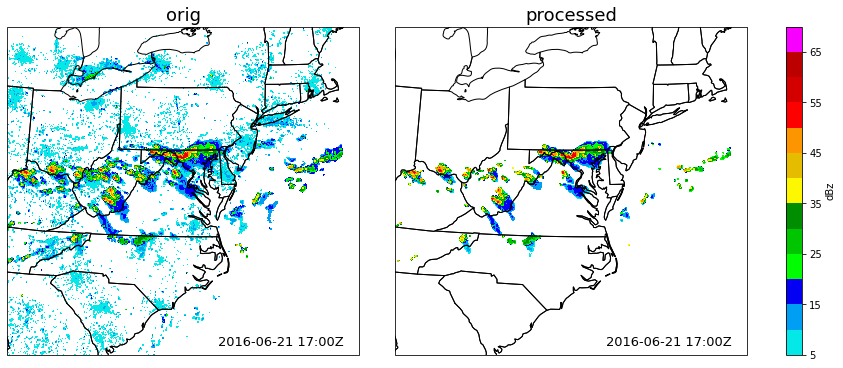
\includegraphics[width=\textwidth]{gridrad_compare}
\singlespacing
\caption{\textit{Gridrad radar composite (column maximum) at 2016-06-21T17:00 before (left) and after (right) filtering and decluttering.}}
\label{fig:gridrad_compare}
\end{figure}

\begin{figure}[H]
\centering
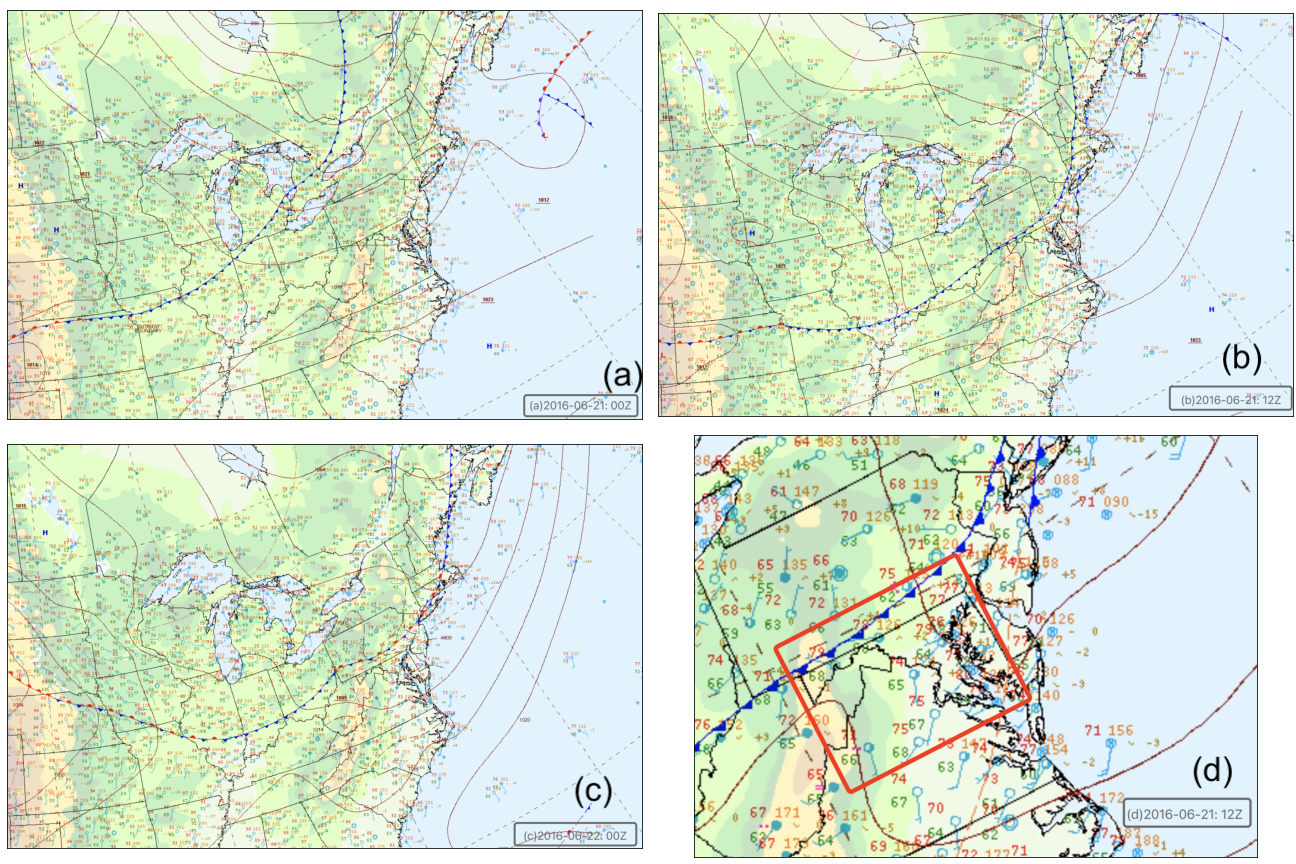
\includegraphics[width=\textwidth]{synoptics}
\singlespacing
\caption{\textit{Surface analysis retrieved from NOAA Weather Forecast Center (WPC, https://www.wpc.ncep.noaa.gov/html/sfc-zoom.php) at (a) 2016-06-21 00Z; (b) 2016-06-21 12Z; (c) 2016-06-22 00Z and (d) 2016-06-21 12Z zoomed in at eastern mid-Atlantic; the red box represents the region of interest}}
\label{fig:synoptics}
\end{figure}

\begin{figure}[H]
\centering
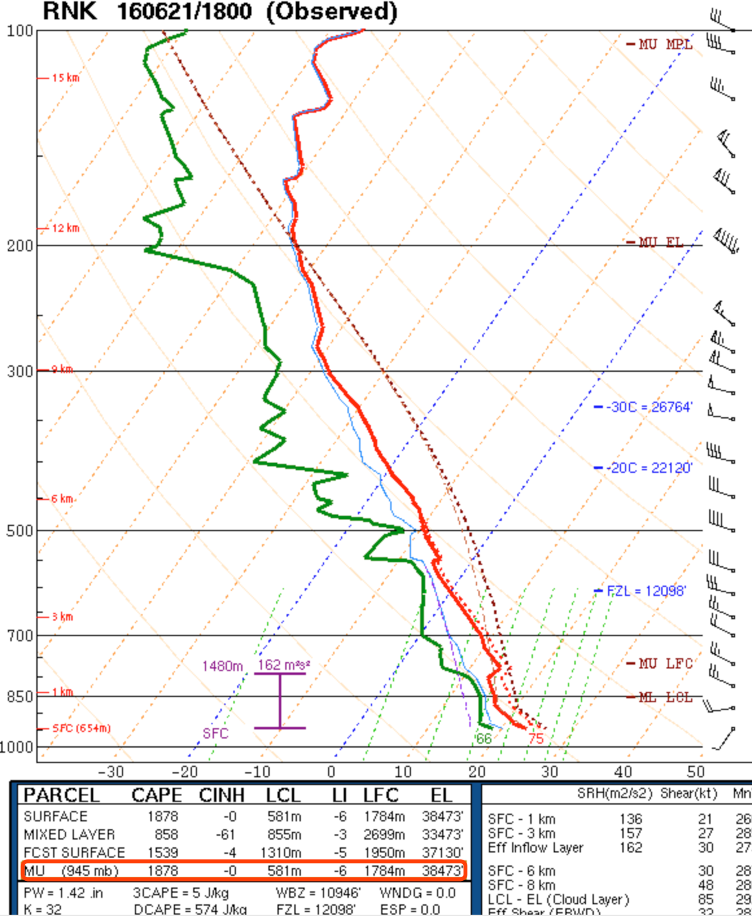
\includegraphics[width=0.7\textwidth]{sounding}
\singlespacing
\caption{\textit{Portion of 18Z sounding plot at Blacksburg, VA from WPC (https://www.spc.noaa.gov/exper/archive/event.php?date=20160621)}}
\label{fig:sounding}
\end{figure}

\begin{figure}[H]
\centering
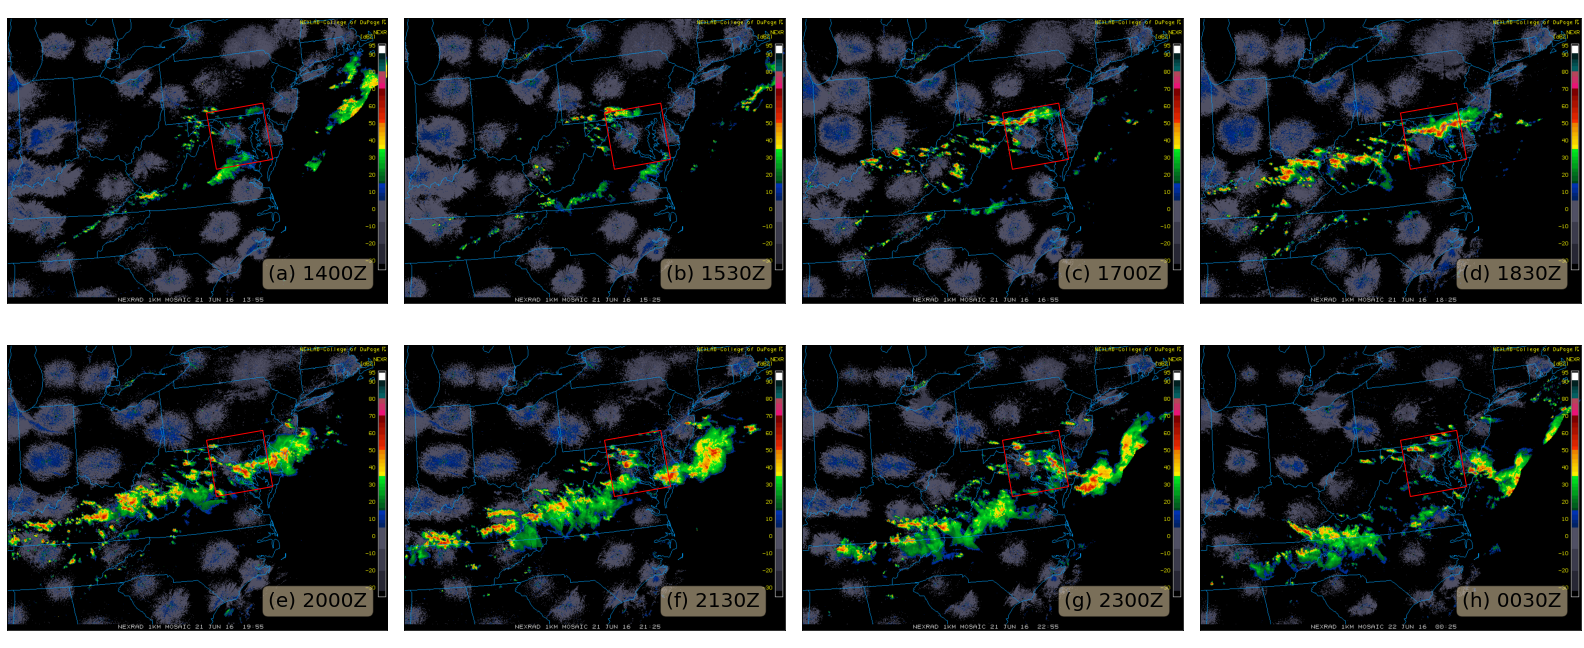
\includegraphics[width=\textwidth]{refs}
\singlespacing
\caption{\textit{Radar composite over the mid-Atlantic with a 1.5-hour interval starting at 2016-06-21 1400Z; the red box represents the region of interest.  Images retrieved from UCAR at https://www2.mmm.ucar.edu/imagearchive}.}
\label{fig:refs}
\end{figure}

\begin{figure}[H]
\centering
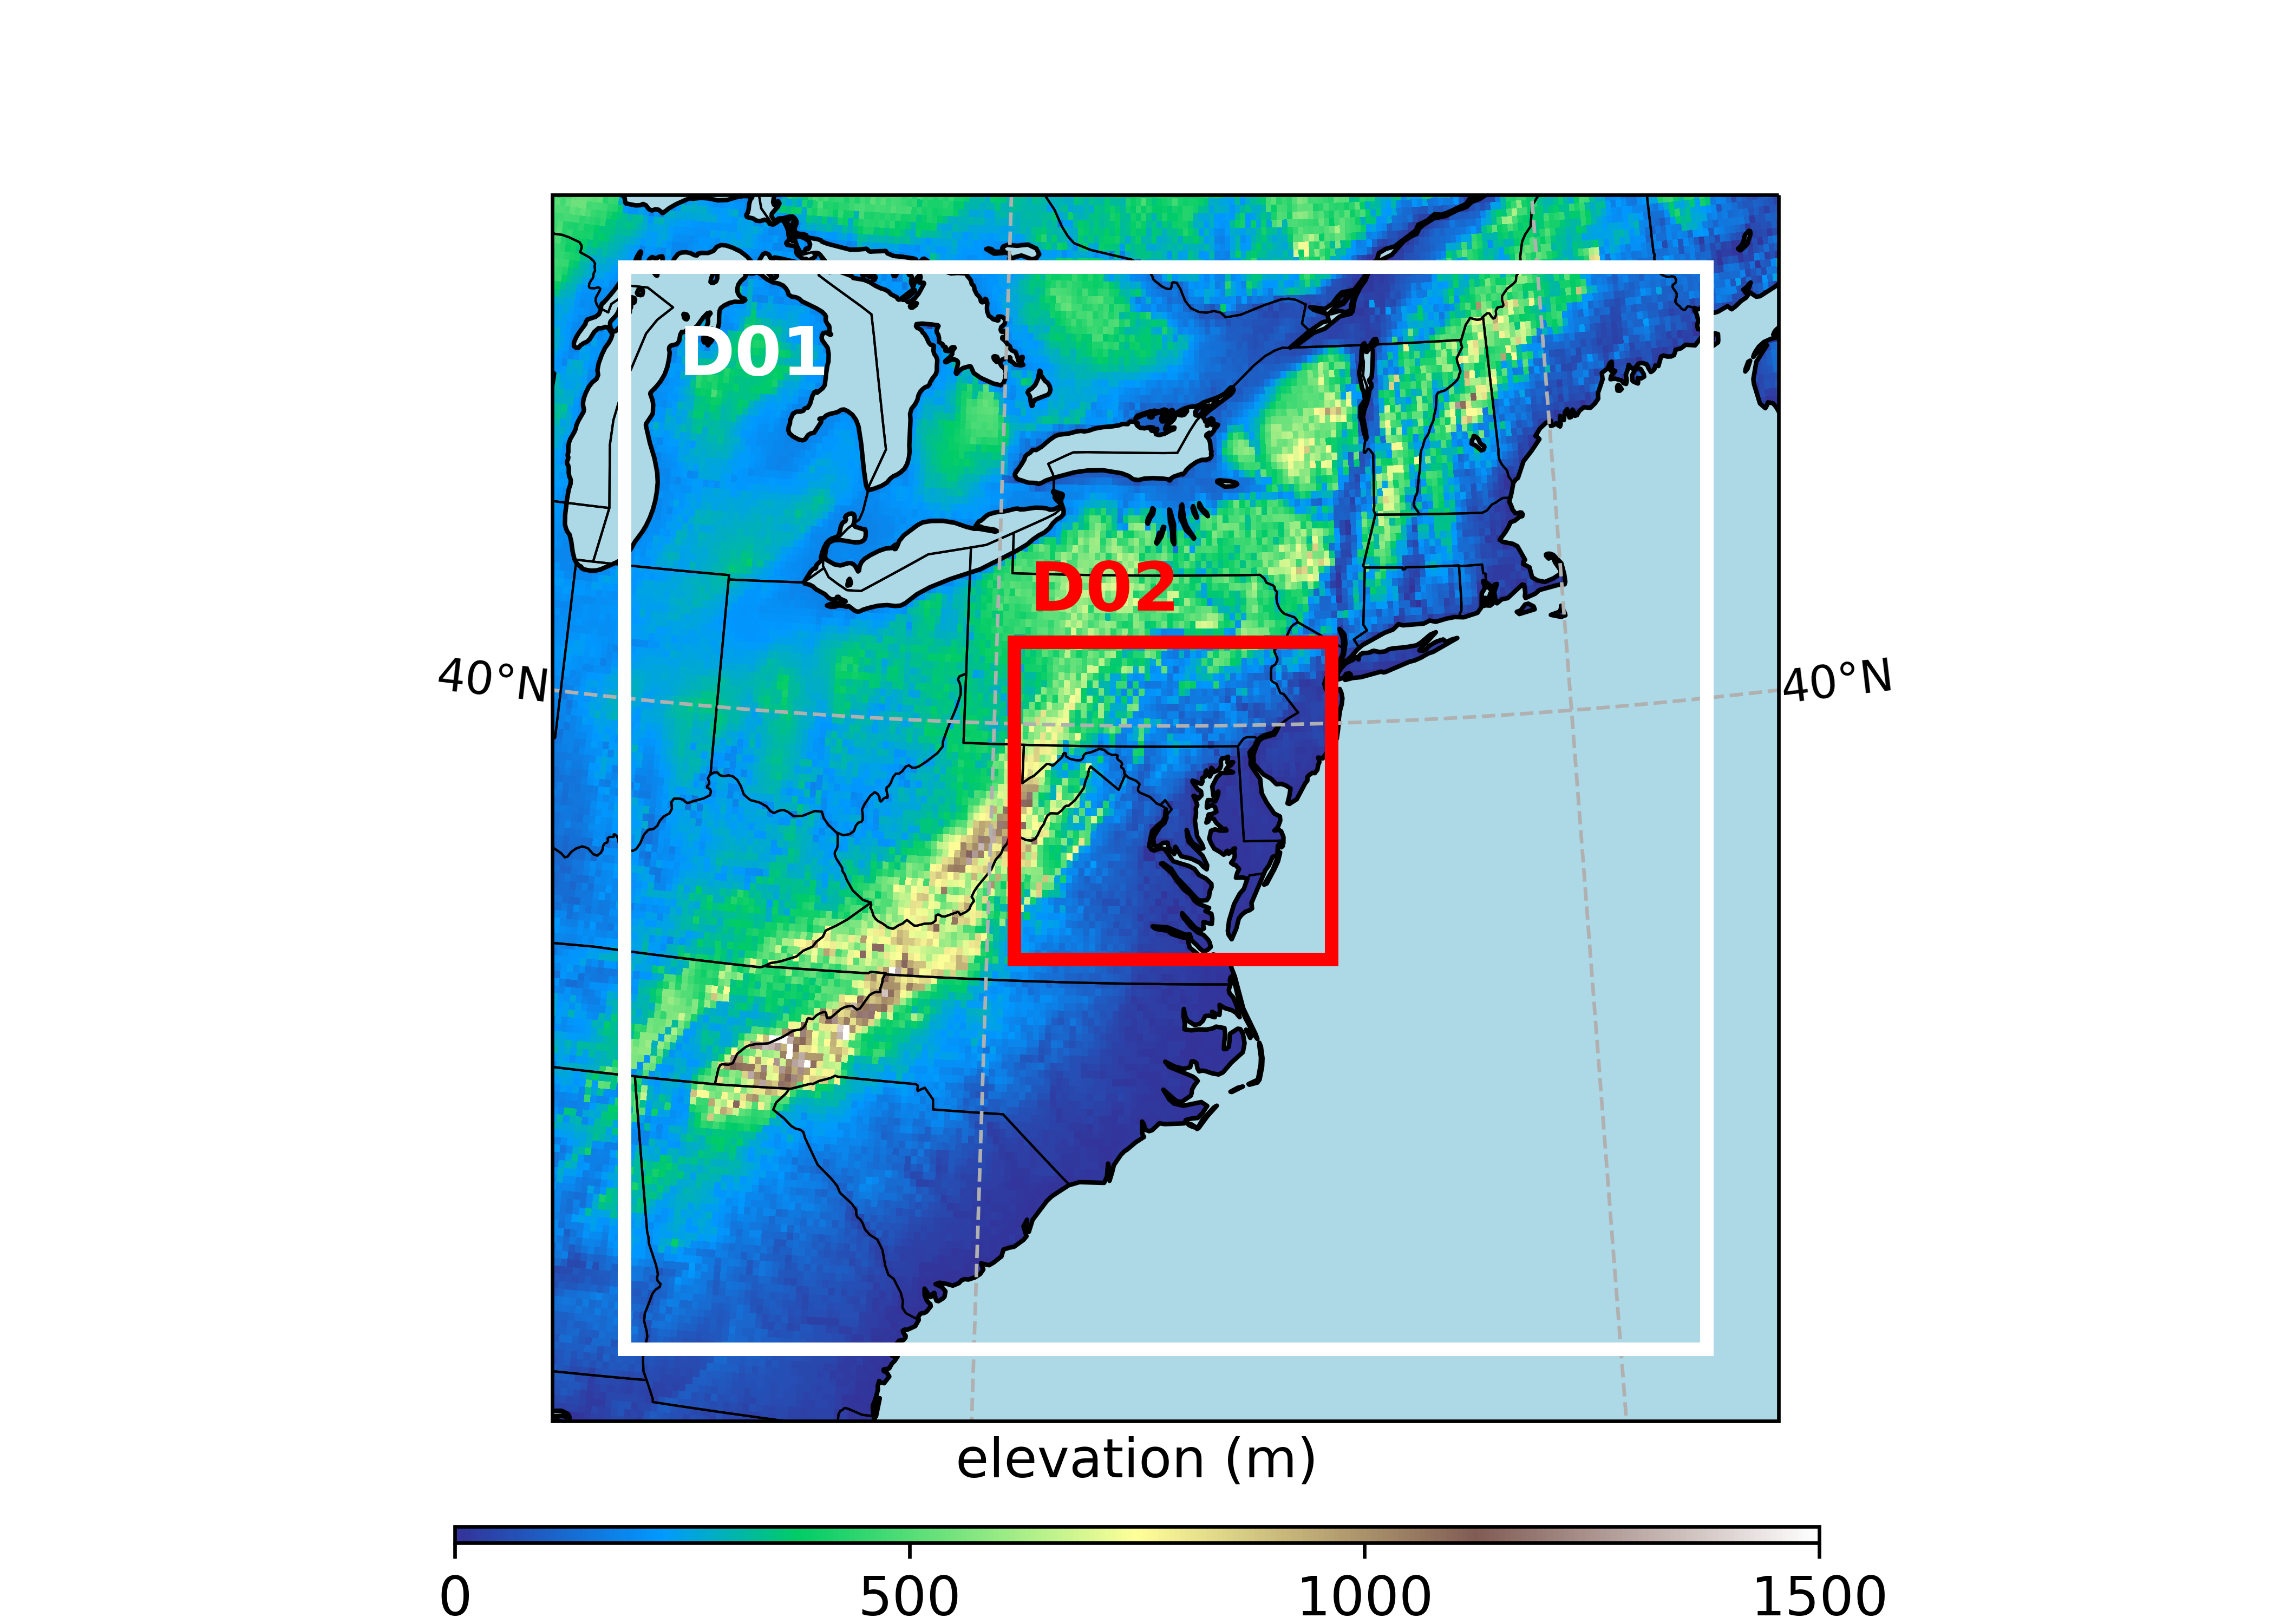
\includegraphics[width=0.85\textwidth]{Domains_20160621_dc}
\singlespacing
\caption{\textit{Domains for all WRF simulation, python script credits to Lucas (https://github.com/lucas-uw/WRF-tools)}}
\label{fig:Domain_2s_20160621_dc}
\end{figure}

\begin{figure}[H]
\centering
\vspace{-20pt}
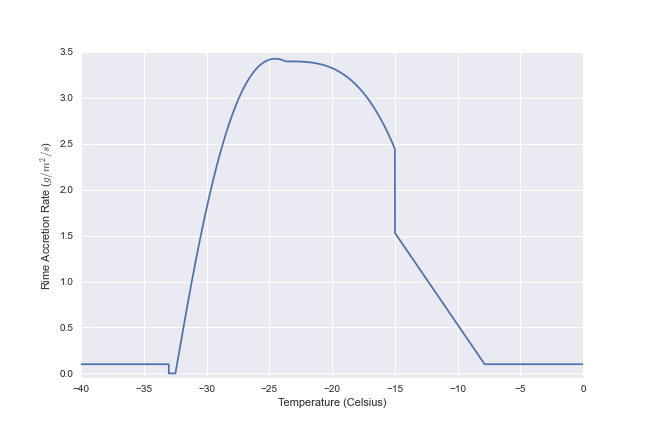
\includegraphics[width=0.85\textwidth]{RAR}
\singlespacing
\vspace{-40pt}
\caption{\textit{Critical RAR as a function of temperature, used in both N2M and M2M}}
\label{fig:RAR}
\end{figure}


\begin{figure}[H]
\centering
% \vspace{-10pt}
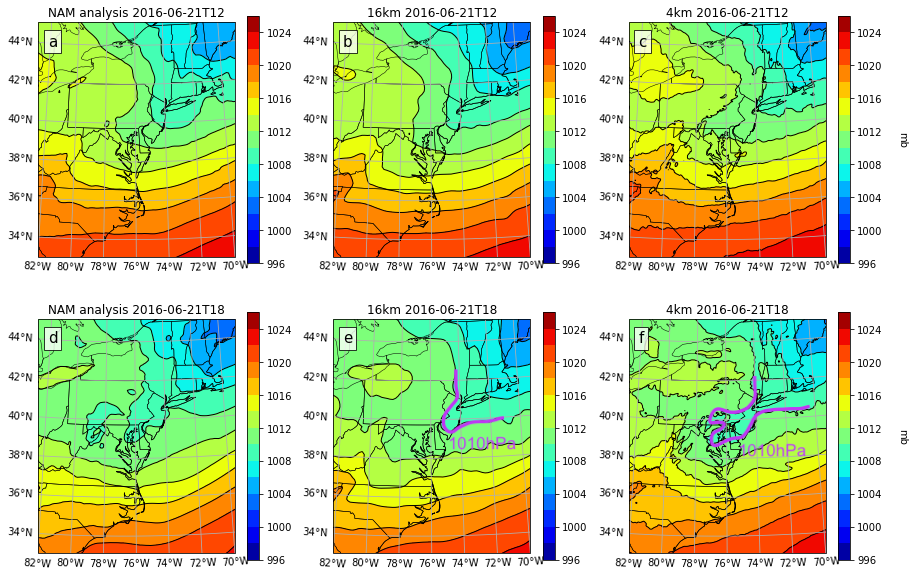
\includegraphics[width=\textwidth]{mslp}
\singlespacing
\vspace{-10pt}
\caption{\textit{Mean Sea Level Pressure (hPa) from NAM reanalysis (a,d) and WRF simulation with 16km (b,e) and 4km (c,f) horizontal resolution at 1200 UTC 21 Jun (a-c) and 1800 UTC 21 Jun (d-f). Same color scheme applied to all subplots.}}
\label{fig:mslp}
\end{figure}

\begin{figure}[H]
\centering
% \vspace{-10pt}
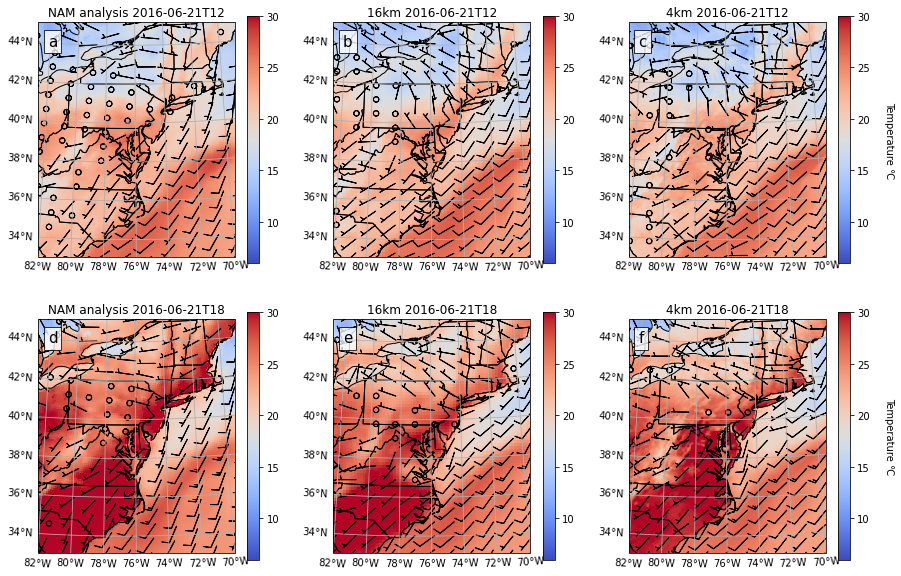
\includegraphics[width=\textwidth]{sfc_analysis}
\singlespacing
\vspace{-10pt}
\caption{\textit{Same as \ref{fig:mslp} but for 2-meter temperature in Celsius (shaded) and 10-meter wind (m/s). Same color scheme applied to all subplots.}}
\label{fig:sfc_analysis}
\end{figure}

\begin{figure}[H]
\centering
% \vspace{-10pt}
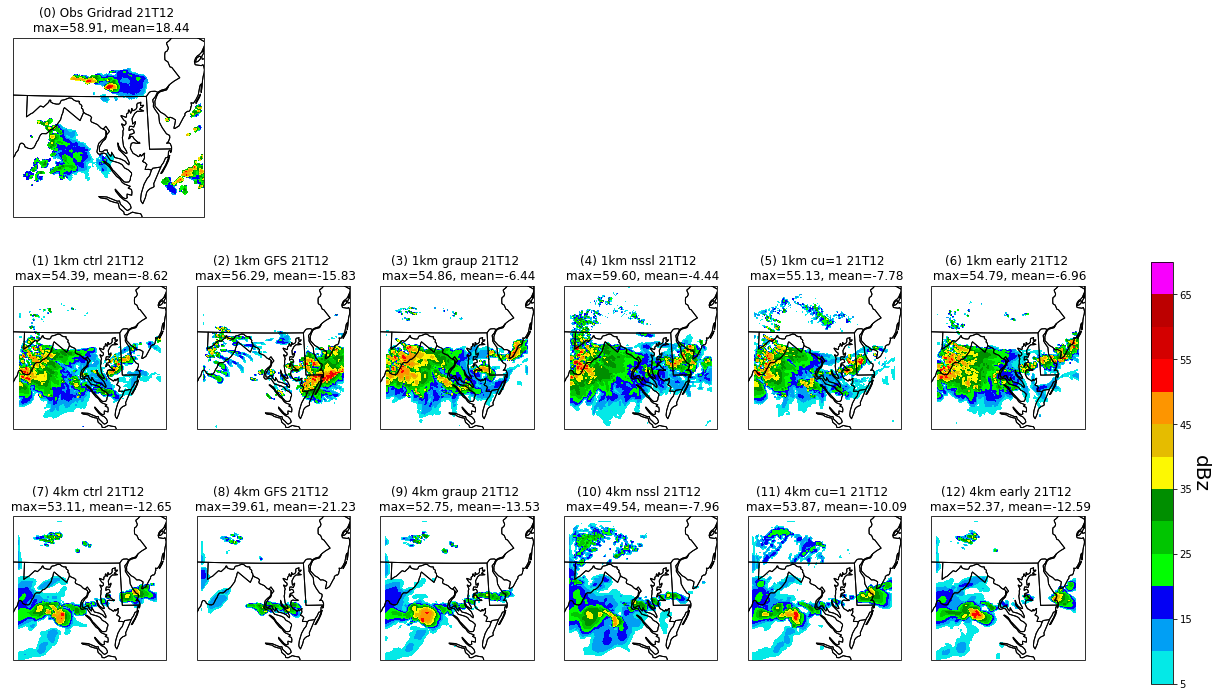
\includegraphics[width=\textwidth]{RadarComposite_2sets_21T12}
\singlespacing
\vspace{-10pt}
\caption{\textit{Radar composite at 1200 UTC 21 Jun 2016 from NEXRAD processed by GridRad (0), and from all 12 simulation members in \ref{table:config}}}
\label{fig:radard02_21T12}
\end{figure}

\begin{figure}[H]
\centering
% \vspace{-10pt}
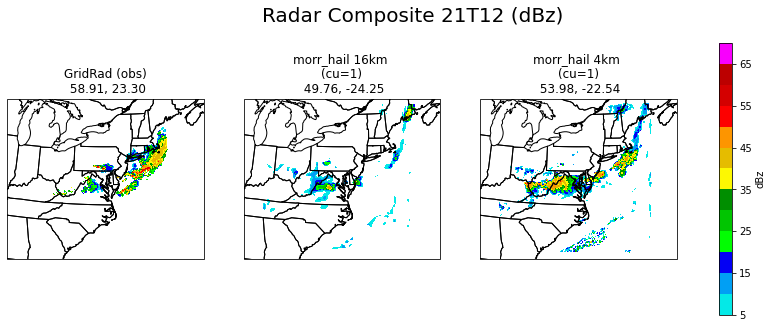
\includegraphics[width=\textwidth]{RadarComposite_d01_21T12}
\singlespacing
\vspace{-10pt}
\caption{\textit{Same as \ref{fig:radard02_21T12} but for the outer domain of member (1) and (7)}}
\label{fig:radard01_21T12}
\end{figure}

\begin{figure}[H]
\centering
% \vspace{-10pt}
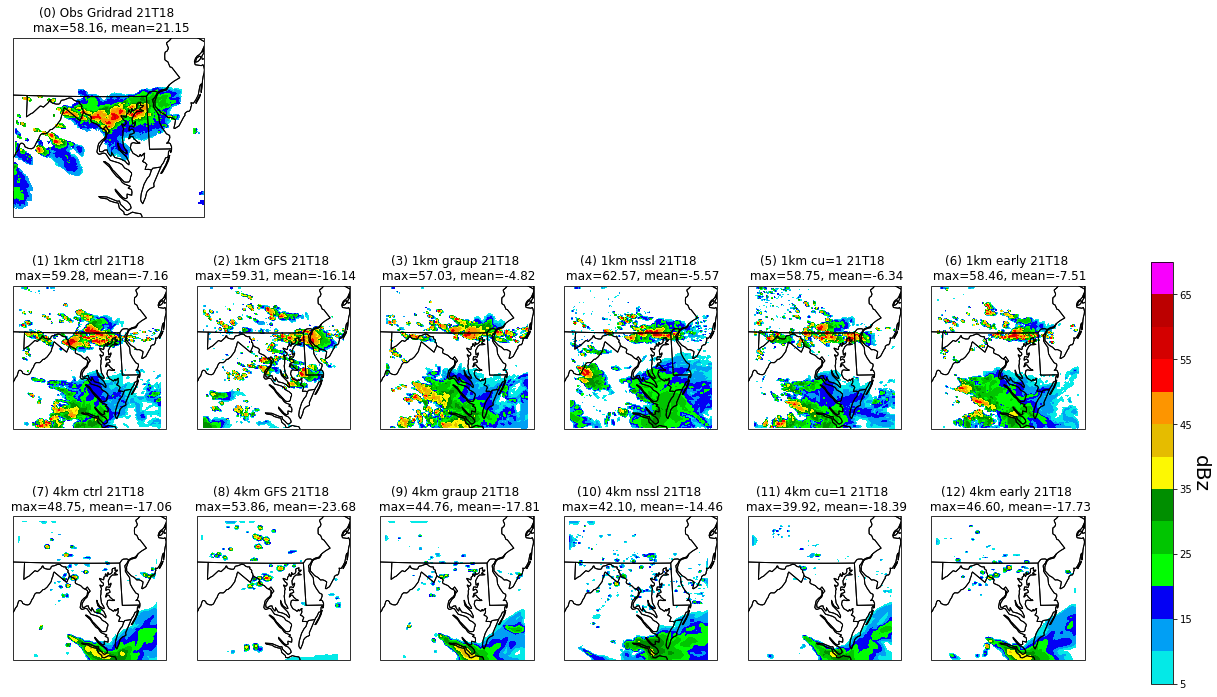
\includegraphics[width=\textwidth]{RadarComposite_2sets_21T18}
\singlespacing
\vspace{-10pt}
\caption{\textit{Same as \ref{fig:radard02_21T12} but for 1800 UTC 21 Jun 2016}}
\label{fig:radard02_21T18}
\end{figure}


\begin{figure}[H]
\centering
% \vspace{-10pt}
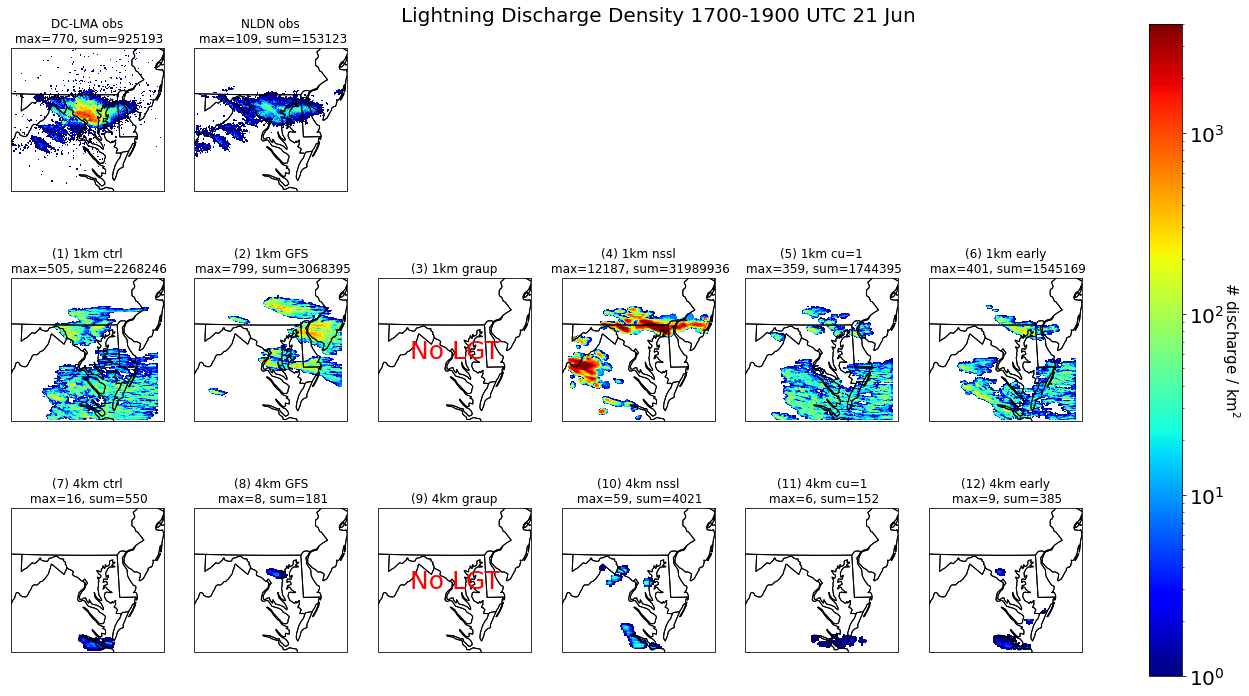
\includegraphics[width=\textwidth]{lightdis_2sets_17-19Z}
\singlespacing
\vspace{-10pt}
\caption{\textit{Lightning discharge density ($\#/km^2$) during 1700-1900 UTC 21 Jun 2016 from DC-LMA and NLDN (top 2 plots) and from 12 members of simulation}}
\label{fig:lightdis17_19}
\end{figure}

\begin{figure}[H]
\centering
% \vspace{-10pt}
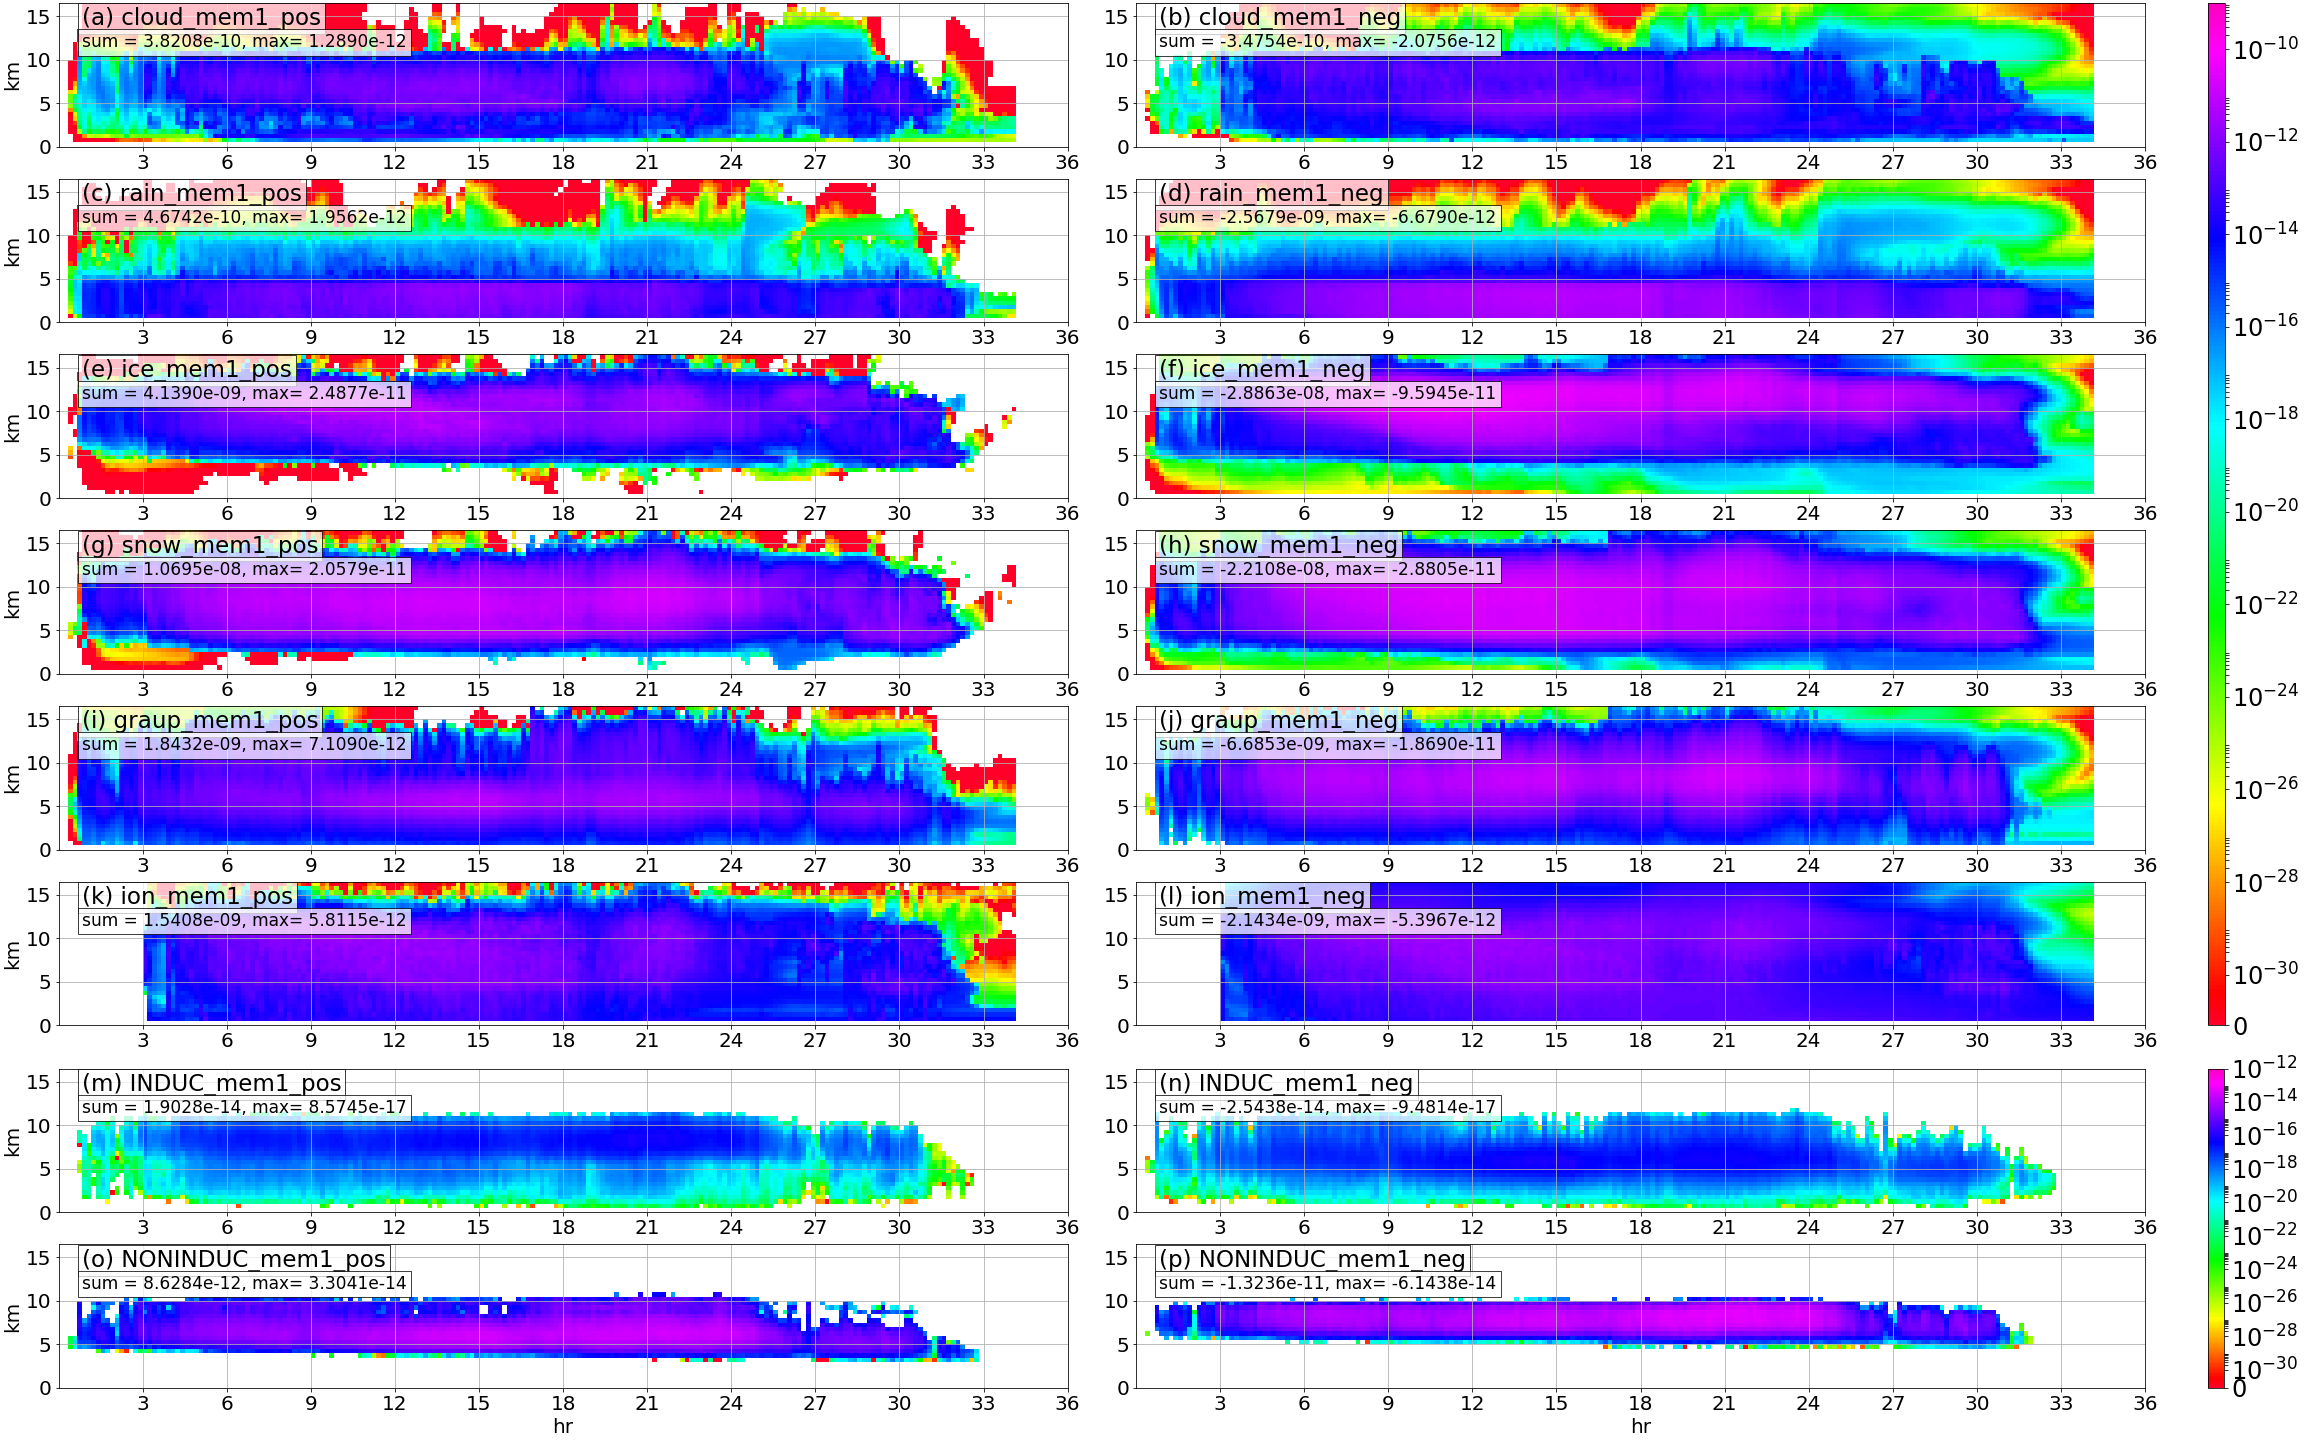
\includegraphics[width=\textwidth]{mem1_scx_crate}
\singlespacing
\vspace{-10pt}
\caption{\textit{Member(1) simulated positive (left) and negative(right) charge carried by cloud(a,b), rain(c,d), ice(e,f), snow(g,h), hail(i,j) and ions(k,l), inductive(m,n) and noninductive(o,p) charging rate, averaged over the domain horizontally, at each 10min timestep and 0.5km layer. Note that the abrupt start of ion charge (k,l) is due to the fact that ion charge is only created as a result of lightning breakdown and charge released from hydrometeors, before which there is currently no explicit scheme parameterized for ion charging.}}
\label{fig:mem1_charge}
\end{figure}

\begin{figure}[H]
\centering
% \vspace{-10pt}
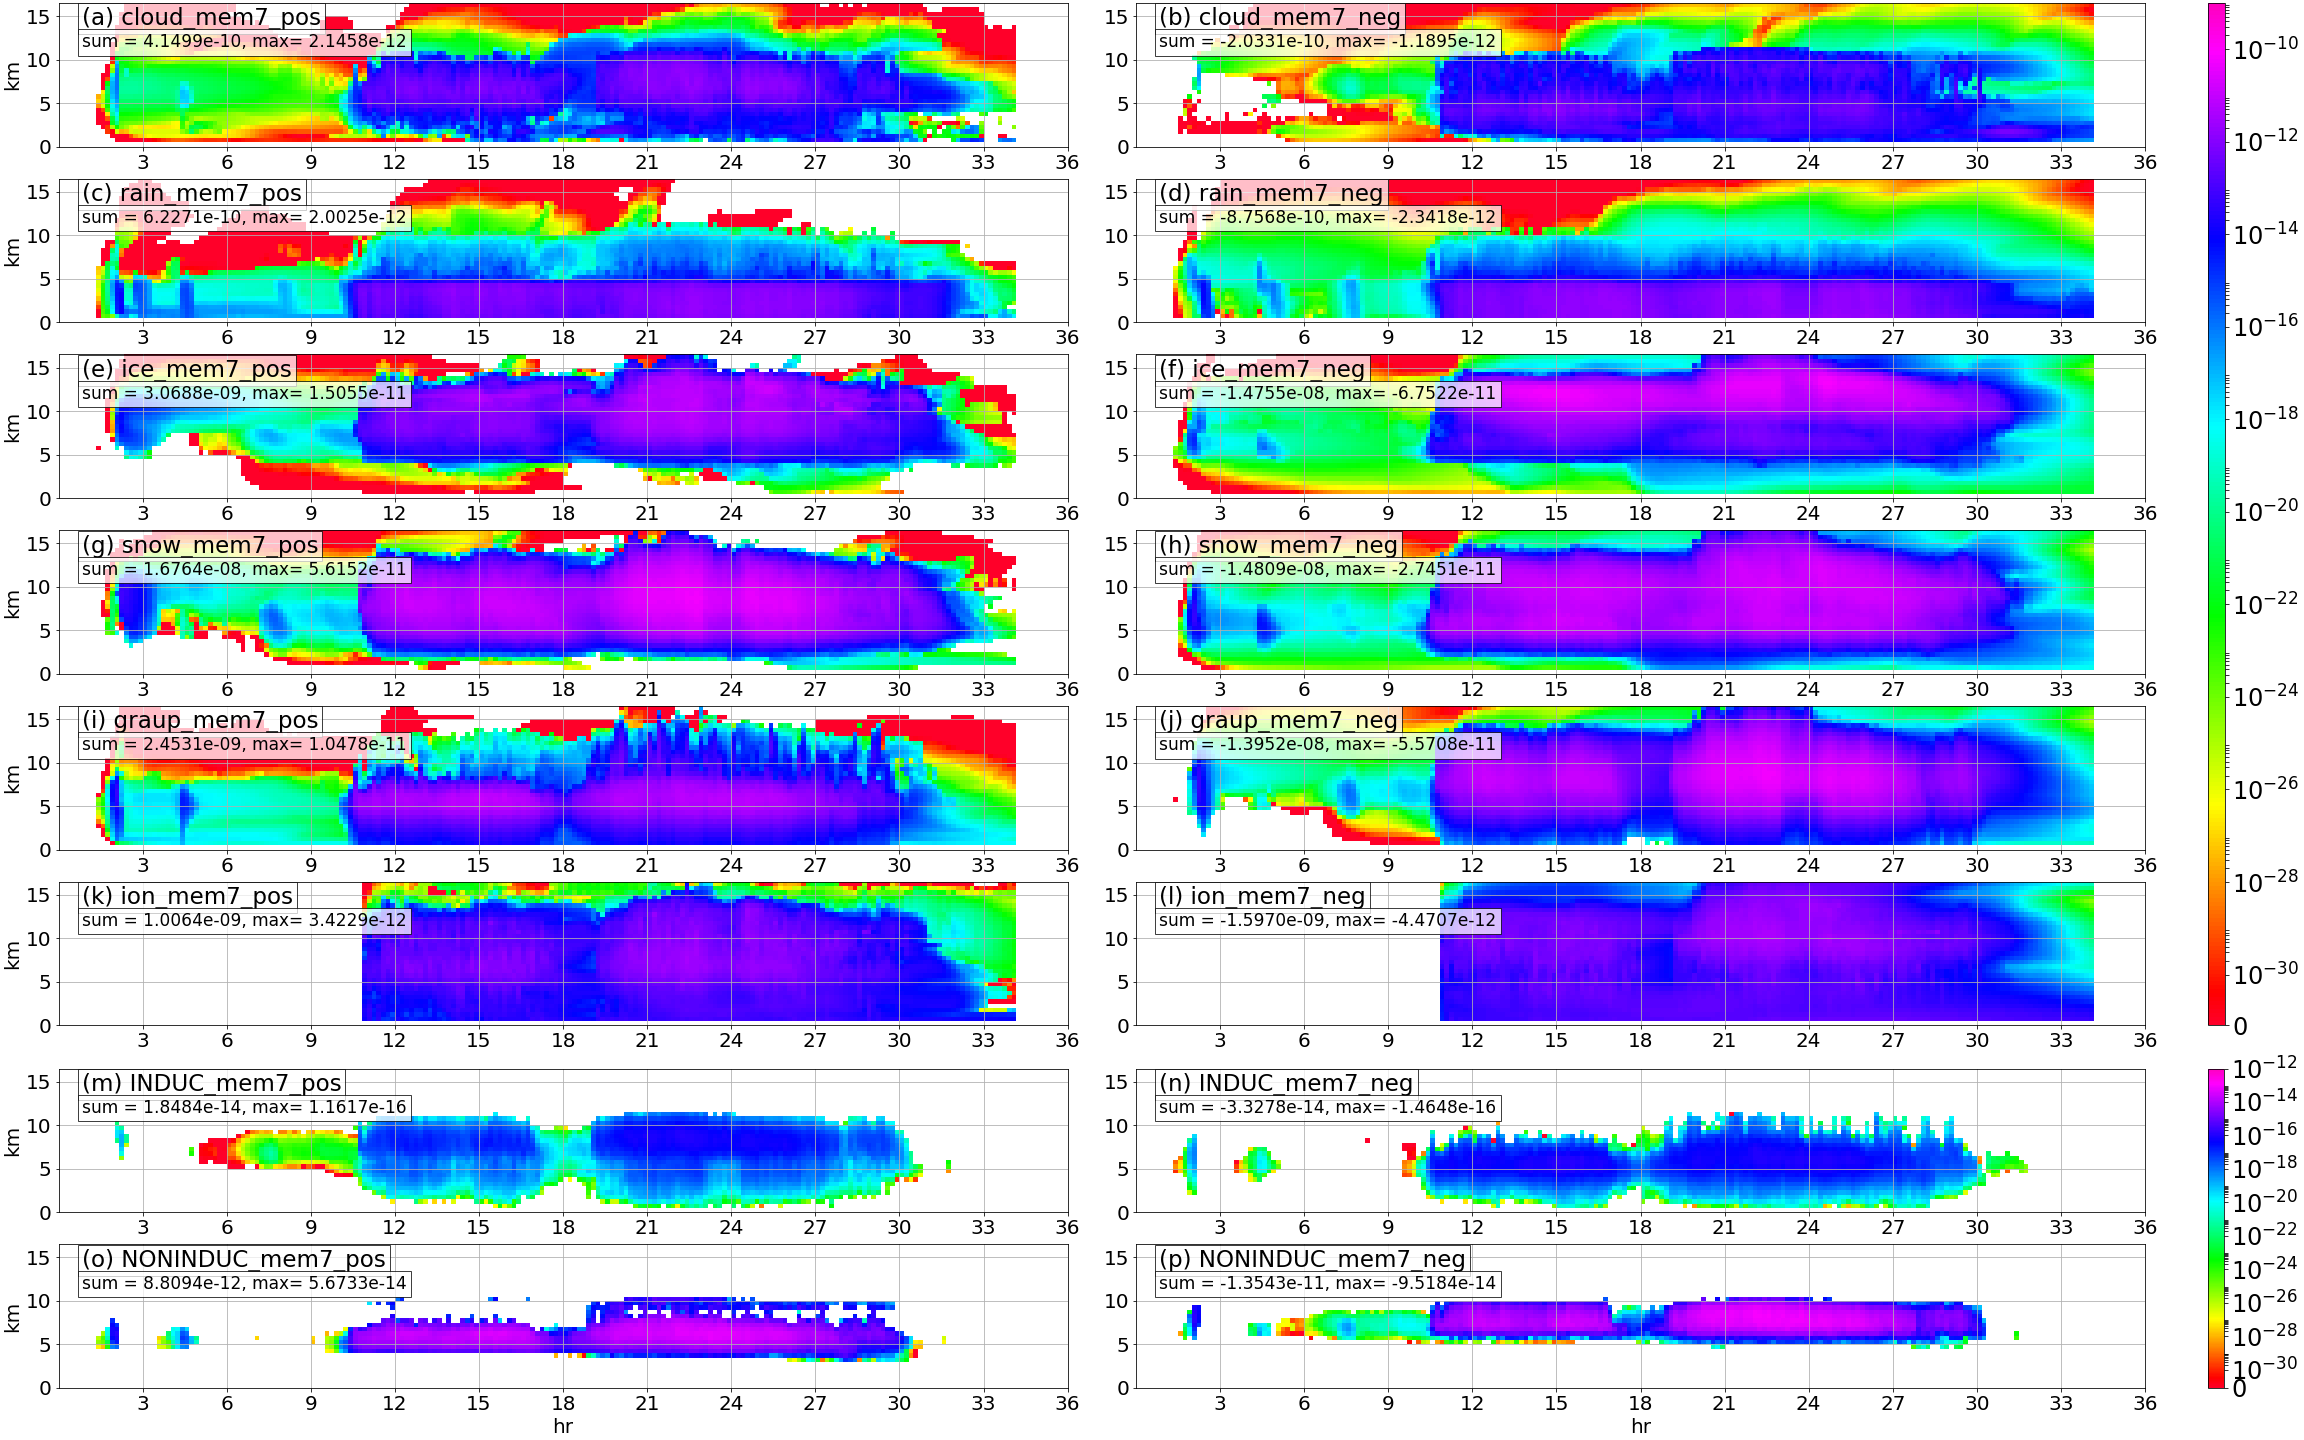
\includegraphics[width=\textwidth]{mem7_scx_crate}
\singlespacing
\vspace{-10pt}
\caption{\textit{Same as \ref{fig:mem1_charge} but for member(7) (4km control run)}}
\label{fig:mem7_charge}
\end{figure}


\begin{figure}[H]
\centering
\vspace{-20pt}
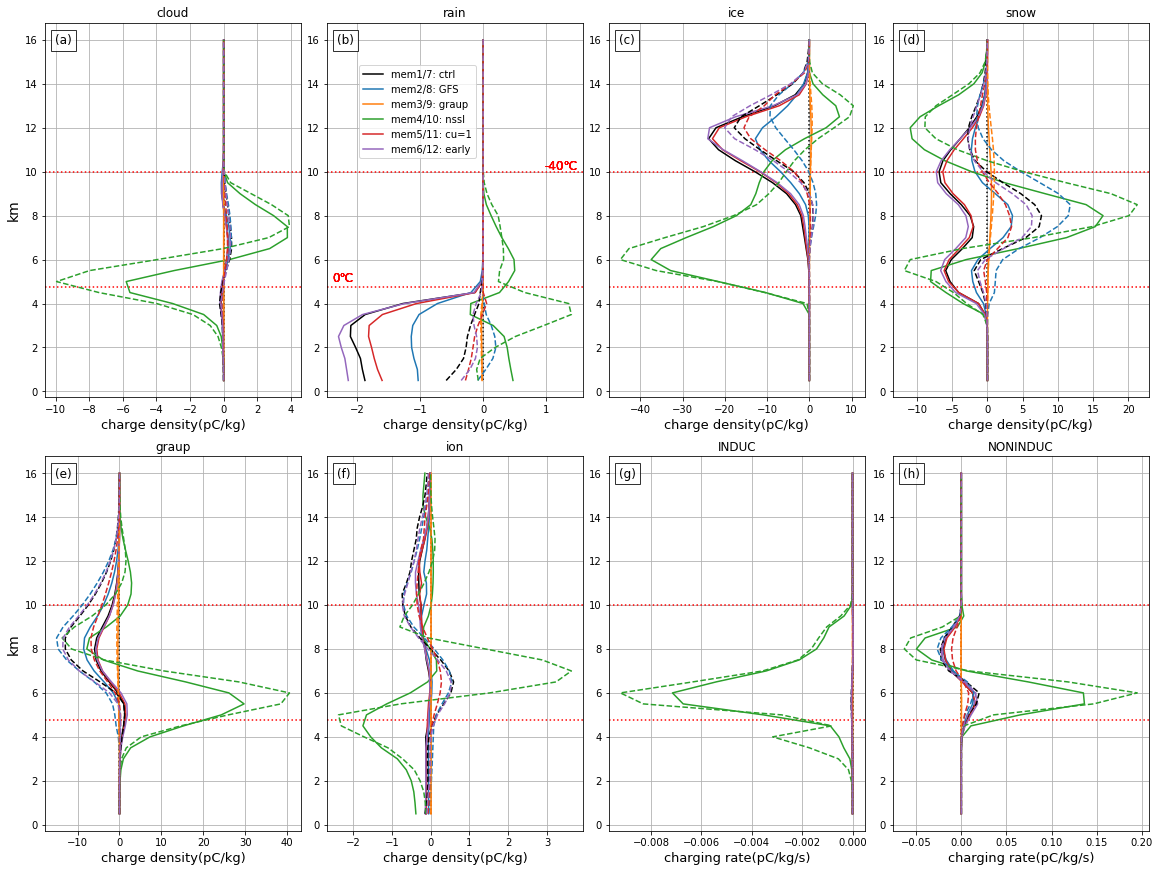
\includegraphics[width=\textwidth]{charge_z1d}
\singlespacing
% \vspace{10pt}
\caption{\textit{Vertical (km) distribution of charge (C/kg) of hydrometeors (a-e), ion(f), inductive(g) and noninductive(h) charging rate, averaged over the horizontal layer and over the 10-30 hour of simulation. Solid lines represent 1km simulation (member 1-6), dashed lines represent 4km (member 7-12), with same colors corresponding to members with analogous settings except for horizontal resolution. Horizontal red dotted lines represent the domain-averaged heights for 0 and -40 Celsius. Refer to \ref{table:config} for more information on members.}}
\label{fig:charge_z1d}
\end{figure}

\begin{figure}[H]
\centering
\vspace{-10pt}
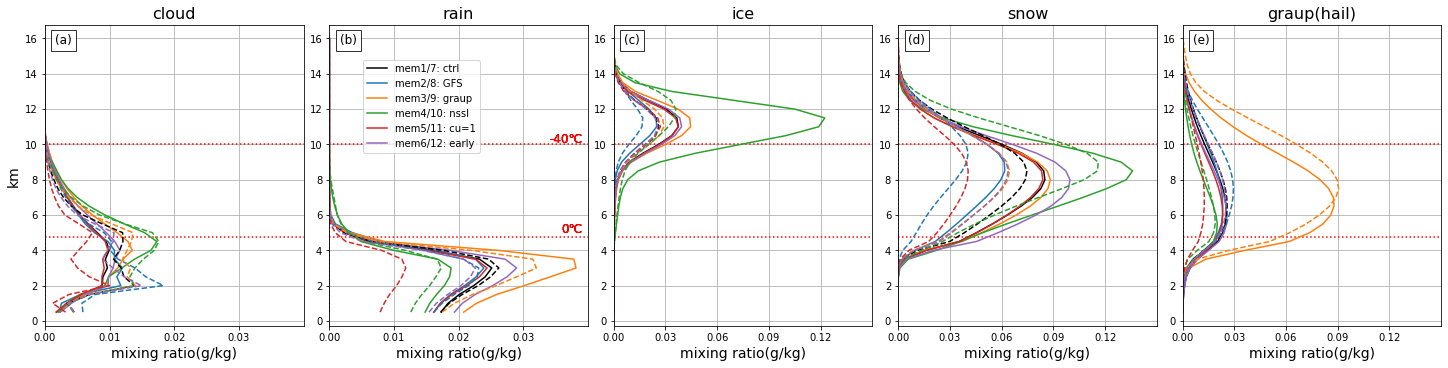
\includegraphics[width=\textwidth]{hdmt_z1d}
\singlespacing
\vspace{-20pt}
\caption{\textit{Vertical distribution of mass mixing ratio (g/kg) of hydrometeors, averaged over the horizontal layer and over the 10-30 hour of simulation. Note the different scaling of x axis for liquid and ice-phase hydrometeors. Line color and style are same as \ref{fig:charge_z1d}. Refer to \ref{table:config} for more information on members.}}
\label{fig:hdmt_z1d}
\end{figure}


\begin{figure}[H]
\centering
\vspace{-10pt}
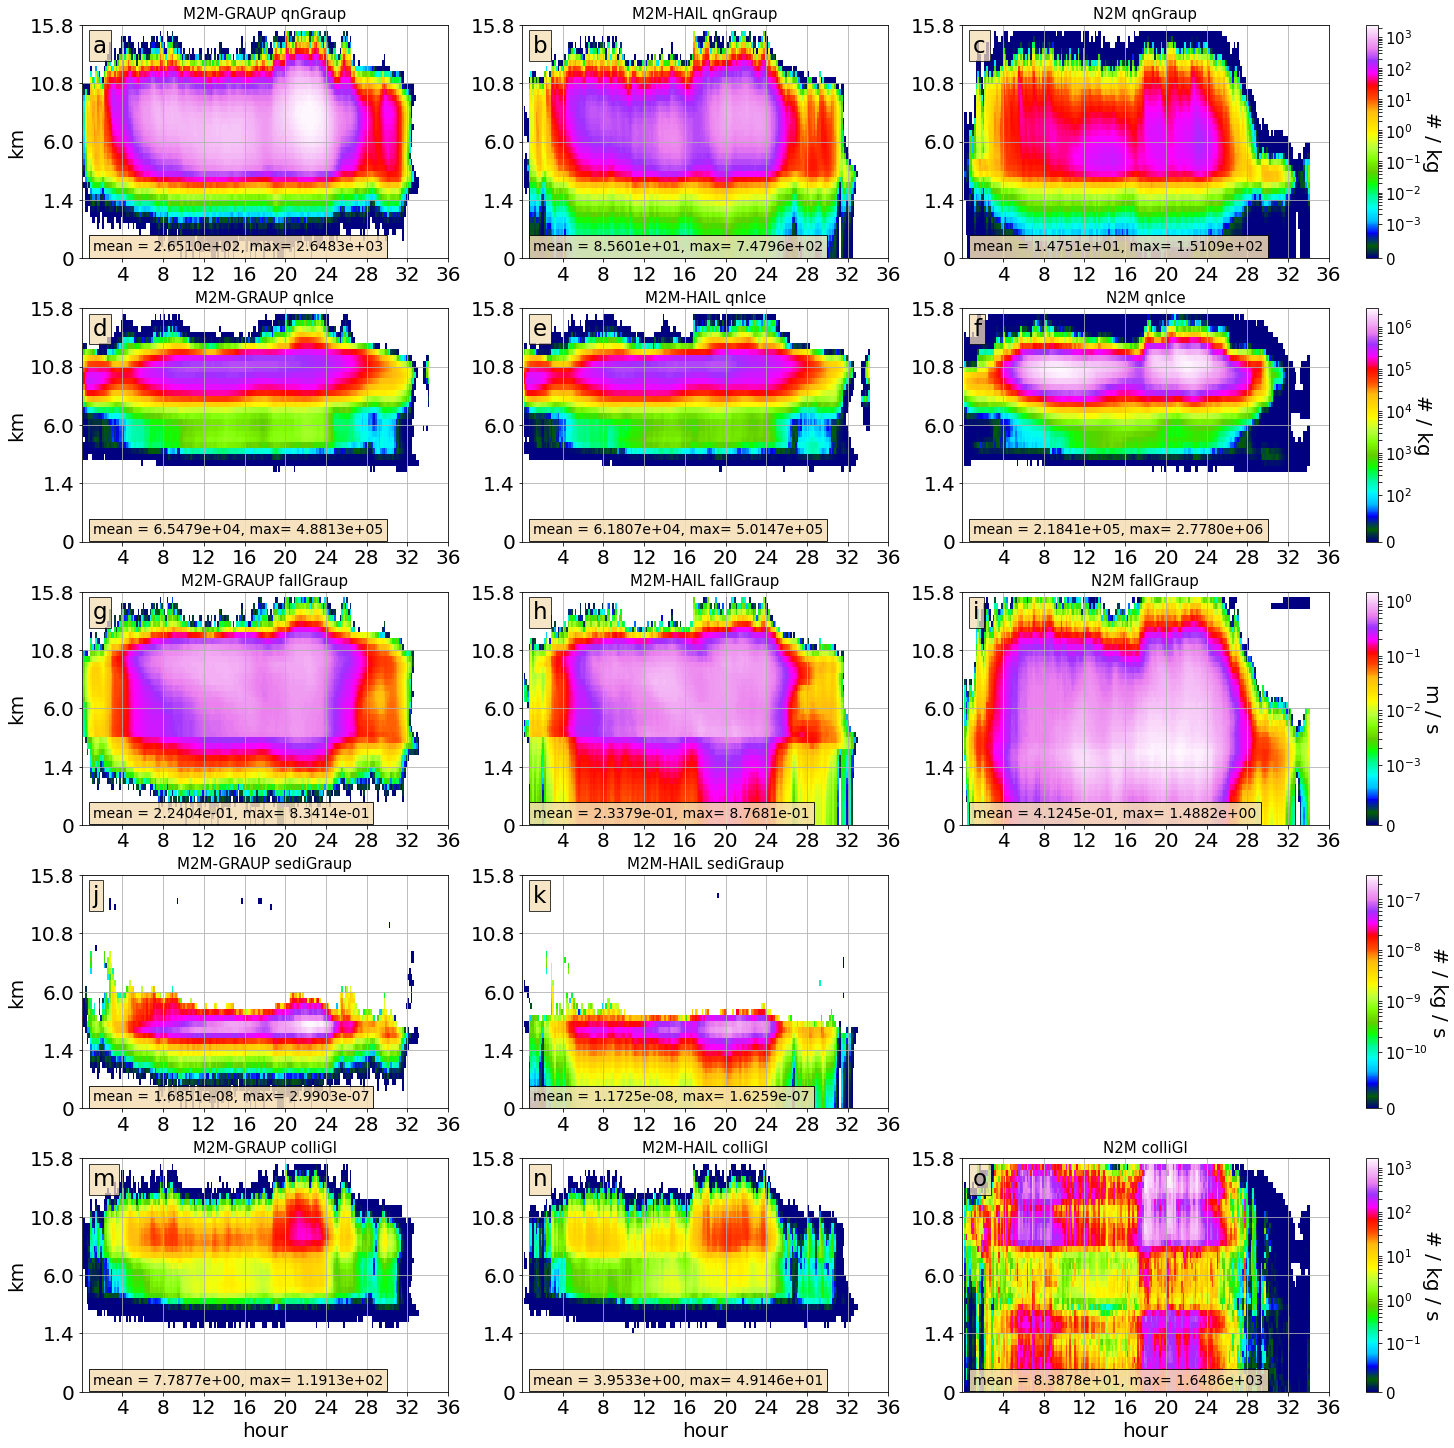
\includegraphics[width=\textwidth]{GIcolli}
\singlespacing
\vspace{-20pt}
\caption{\textit{Time(hour)-height(model level) distribution of horizontally averaged graupel(a-c) and ice(d-f) number mixing ratio in $\#/kg$, graupel fall speed(g-i) in $m/s$, graupel sedimentation rate(j,k) in $\#/kg/s$, and graupel-ice collision rate(m-o) in $\#/kg/s$. The three columns correspond to mem3(1km M2M graupel), mem1(1km M2M ctrl) and mem4(1km N2M), respectively. The graupel sedimentation rate N2M is not yet available and will be added soon.}}
\label{fig:GIcolli}
\end{figure}

\begin{figure}[H]
\centering
\vspace{-10pt}
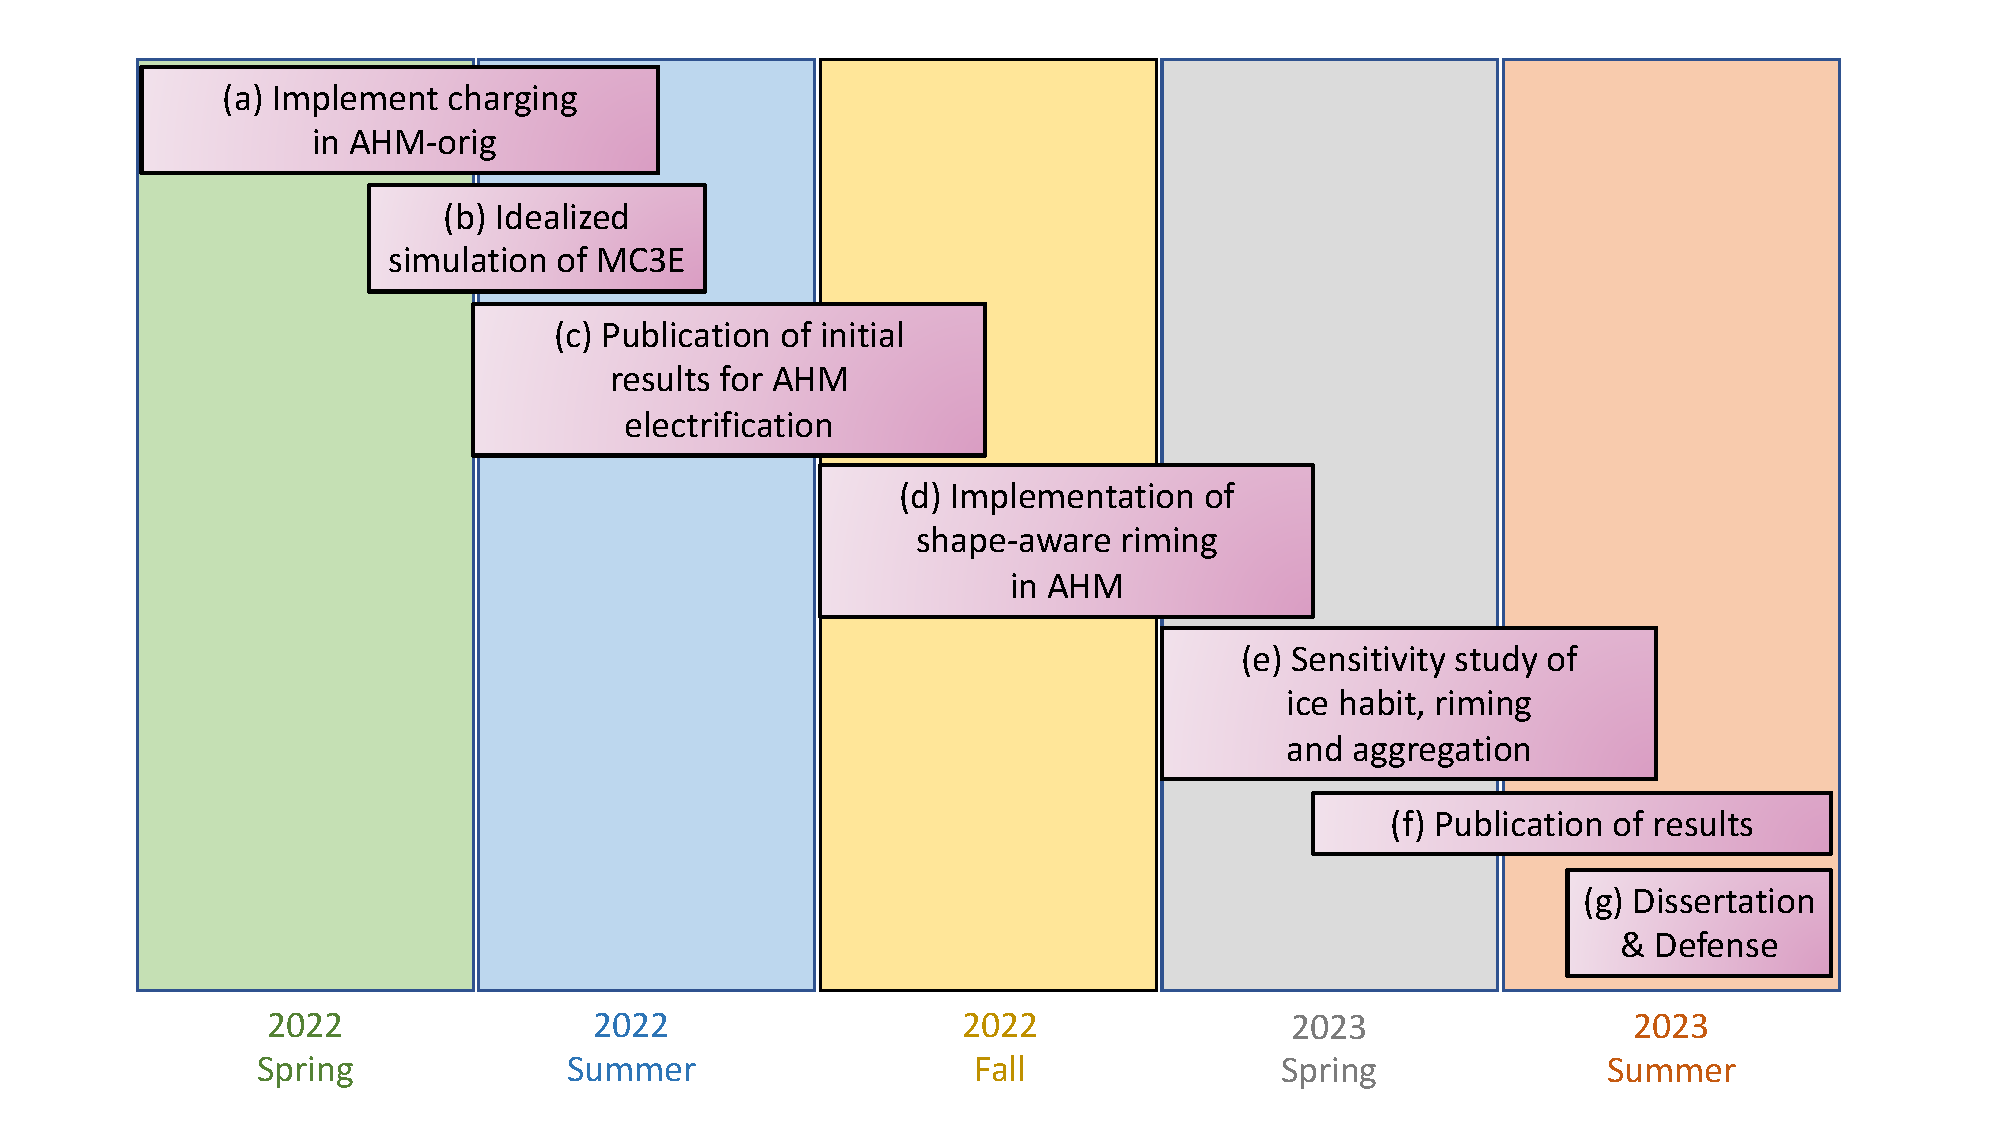
\includegraphics[width=\textwidth]{gantt}
\singlespacing
\vspace{-20pt}
\caption{\textit{Research timeline}}
\label{fig:gantt}
\end{figure}